\documentclass{standalone}
\usepackage{tikz}
\usetikzlibrary{patterns}
\usetikzlibrary{positioning}
\usetikzlibrary{patterns, positioning}
\usetikzlibrary{shapes.misc}
\usepackage[outline]{contour}
\contourlength{1.5pt} 
\usepackage[sfdefault]{ClearSans}

\begin{document}
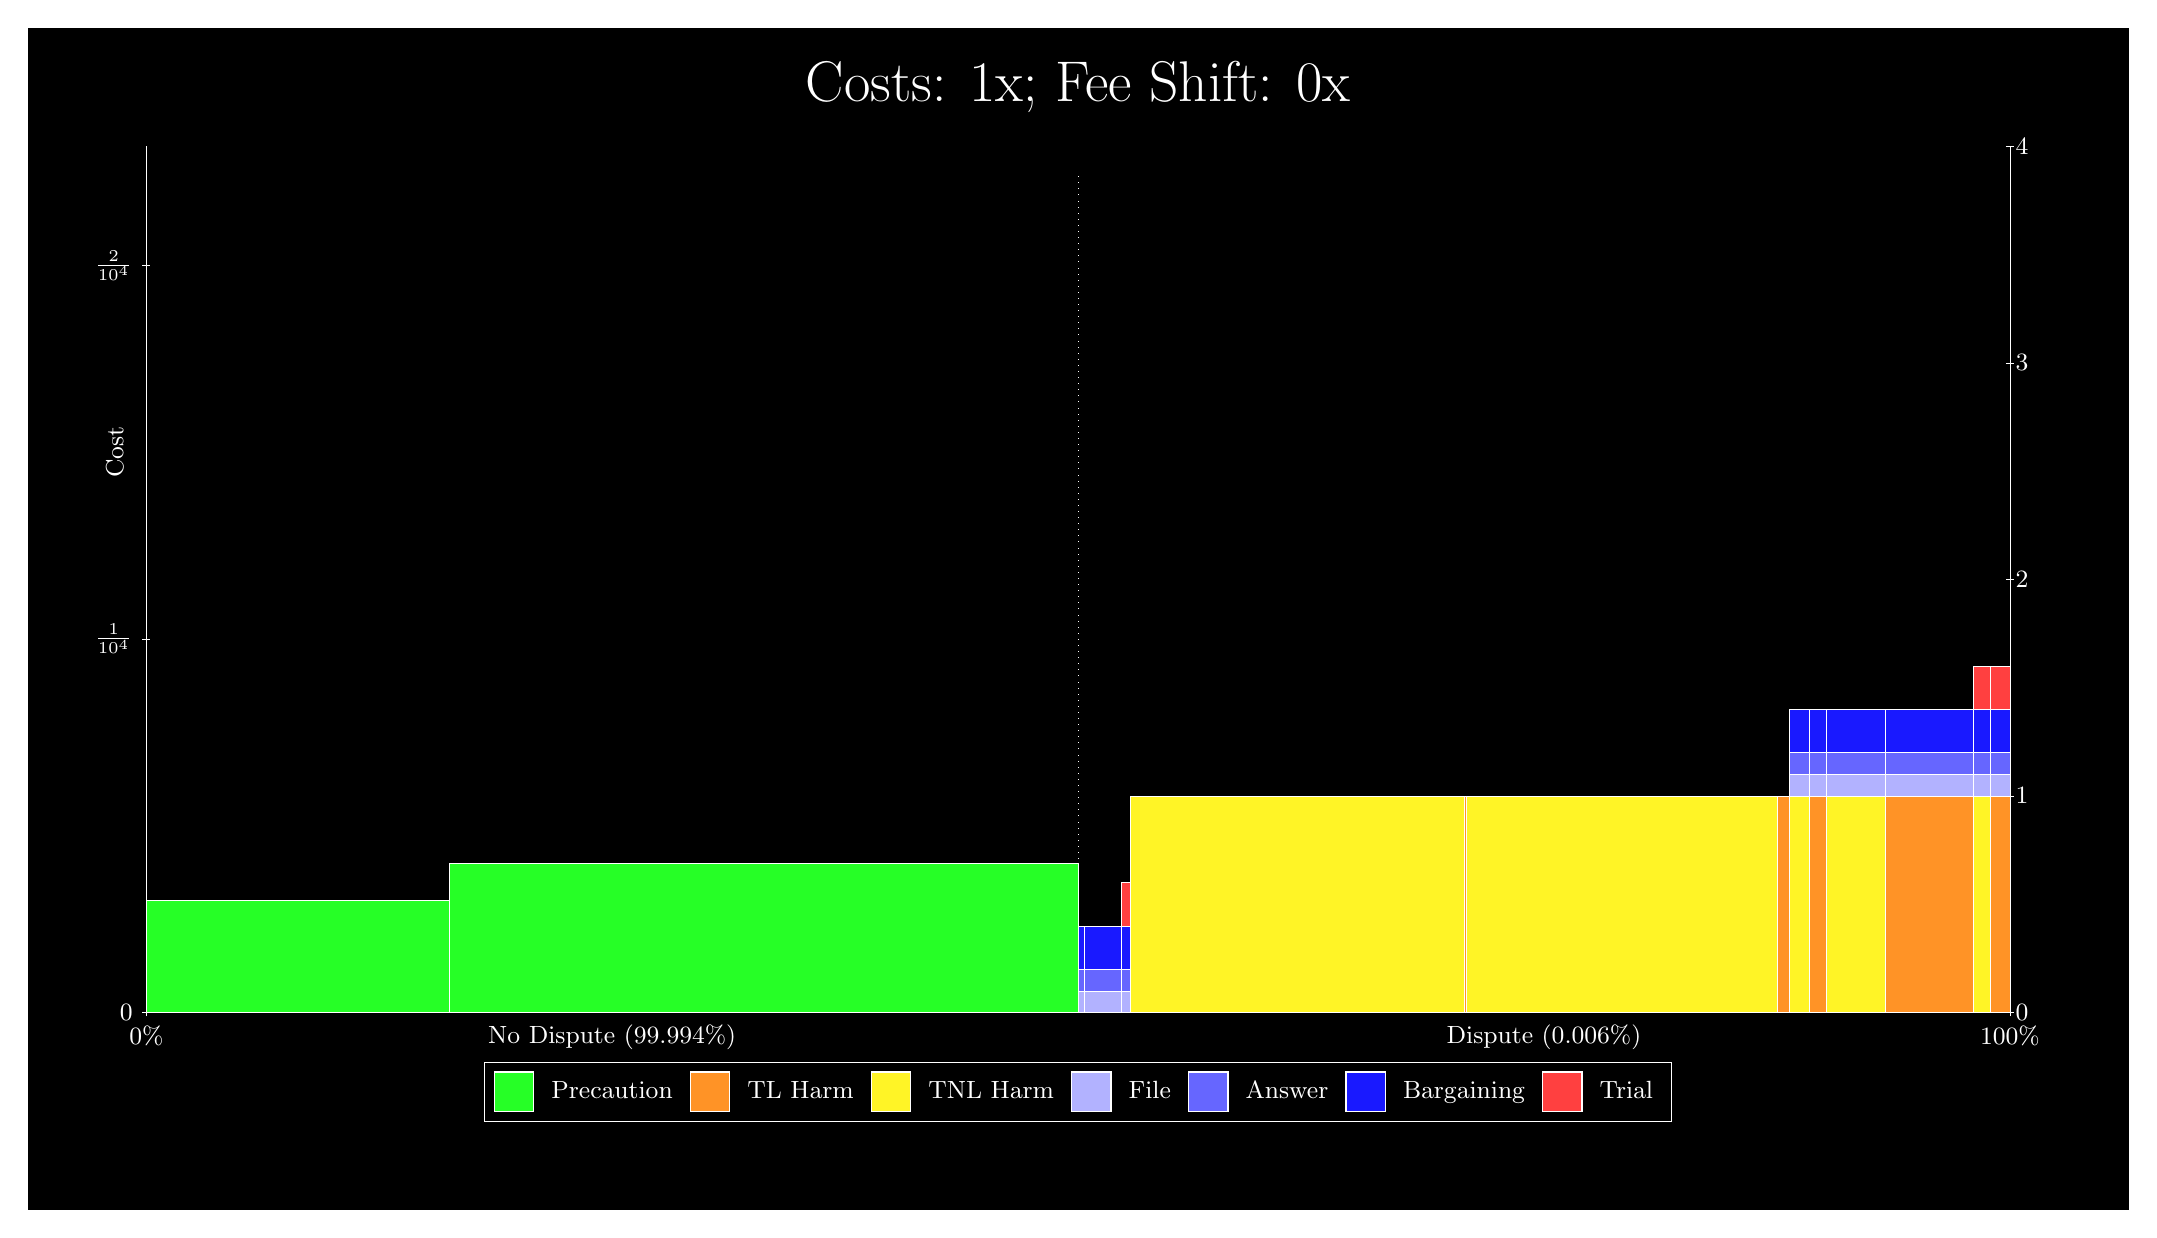
\begin{tikzpicture}
\draw[fill=black] (0,0) rectangle (26.667,15);
\draw[draw=none,text=white] (0,13.5) rectangle (26.667,15) node[midway] {\huge Costs: 1x; Fee Shift: 0x };
\draw[fill=green!85,draw=white,very thin] (1.5,2.5) rectangle (5.3486,3.9232);
\draw[fill=green!85,draw=white,very thin] (5.3486,2.5) rectangle (13.333,4.3976);
\draw[fill=green!85,draw=white,very thin] (13.333,2.5) rectangle (13.407,2.5001);
\draw[fill=blue!30,draw=white,very thin] (13.333,2.5001) rectangle (13.407,2.7751);
\draw[fill=blue!60,draw=white,very thin] (13.333,2.7751) rectangle (13.407,3.0501);
\draw[fill=blue!90,draw=white,very thin] (13.333,3.0501) rectangle (13.407,3.6001);
\draw[fill=green!85,draw=white,very thin] (13.407,2.5) rectangle (13.884,2.5001);
\draw[fill=blue!30,draw=white,very thin] (13.407,2.5001) rectangle (13.884,2.7751);
\draw[fill=blue!60,draw=white,very thin] (13.407,2.7751) rectangle (13.884,3.0501);
\draw[fill=blue!90,draw=white,very thin] (13.407,3.0501) rectangle (13.884,3.6001);
\draw[fill=green!85,draw=white,very thin] (13.884,2.5) rectangle (14.001,2.5001);
\draw[fill=blue!30,draw=white,very thin] (13.884,2.5001) rectangle (14.001,2.7751);
\draw[fill=blue!60,draw=white,very thin] (13.884,2.7751) rectangle (14.001,3.0501);
\draw[fill=blue!90,draw=white,very thin] (13.884,3.0501) rectangle (14.001,3.6001);
\draw[fill=red!75,draw=white,very thin] (13.884,3.6001) rectangle (14.001,4.1501);
\draw[fill=green!85,draw=white,very thin] (14.001,2.5) rectangle (18.237,2.5001);
\draw[fill=yellow!85,draw=white,very thin] (14.001,2.5001) rectangle (18.237,5.2501);
\draw[fill=green!85,draw=white,very thin] (18.237,2.5) rectangle (18.267,2.5001);
\draw[fill=orange!85,draw=white,very thin] (18.237,2.5001) rectangle (18.267,5.2501);
\draw[fill=green!85,draw=white,very thin] (18.267,2.5) rectangle (22.207,2.5001);
\draw[fill=yellow!85,draw=white,very thin] (18.267,2.5001) rectangle (22.207,5.2501);
\draw[fill=green!85,draw=white,very thin] (22.207,2.5) rectangle (22.365,2.5001);
\draw[fill=orange!85,draw=white,very thin] (22.207,2.5001) rectangle (22.365,5.2501);
\draw[fill=green!85,draw=white,very thin] (22.365,2.5) rectangle (22.62,2.5001);
\draw[fill=yellow!85,draw=white,very thin] (22.365,2.5001) rectangle (22.62,5.2501);
\draw[fill=blue!30,draw=white,very thin] (22.365,5.2501) rectangle (22.62,5.5251);
\draw[fill=blue!60,draw=white,very thin] (22.365,5.5251) rectangle (22.62,5.8001);
\draw[fill=blue!90,draw=white,very thin] (22.365,5.8001) rectangle (22.62,6.3501);
\draw[fill=green!85,draw=white,very thin] (22.62,2.5) rectangle (22.84,2.5001);
\draw[fill=orange!85,draw=white,very thin] (22.62,2.5001) rectangle (22.84,5.2501);
\draw[fill=blue!30,draw=white,very thin] (22.62,5.2501) rectangle (22.84,5.5251);
\draw[fill=blue!60,draw=white,very thin] (22.62,5.5251) rectangle (22.84,5.8001);
\draw[fill=blue!90,draw=white,very thin] (22.62,5.8001) rectangle (22.84,6.3501);
\draw[fill=green!85,draw=white,very thin] (22.84,2.5) rectangle (23.581,2.5001);
\draw[fill=yellow!85,draw=white,very thin] (22.84,2.5001) rectangle (23.581,5.2501);
\draw[fill=blue!30,draw=white,very thin] (22.84,5.2501) rectangle (23.581,5.5251);
\draw[fill=blue!60,draw=white,very thin] (22.84,5.5251) rectangle (23.581,5.8001);
\draw[fill=blue!90,draw=white,very thin] (22.84,5.8001) rectangle (23.581,6.3501);
\draw[fill=green!85,draw=white,very thin] (23.581,2.5) rectangle (24.704,2.5001);
\draw[fill=orange!85,draw=white,very thin] (23.581,2.5001) rectangle (24.704,5.2501);
\draw[fill=blue!30,draw=white,very thin] (23.581,5.2501) rectangle (24.704,5.5251);
\draw[fill=blue!60,draw=white,very thin] (23.581,5.5251) rectangle (24.704,5.8001);
\draw[fill=blue!90,draw=white,very thin] (23.581,5.8001) rectangle (24.704,6.3501);
\draw[fill=green!85,draw=white,very thin] (24.704,2.5) rectangle (24.915,2.5001);
\draw[fill=yellow!85,draw=white,very thin] (24.704,2.5001) rectangle (24.915,5.2501);
\draw[fill=blue!30,draw=white,very thin] (24.704,5.2501) rectangle (24.915,5.5251);
\draw[fill=blue!60,draw=white,very thin] (24.704,5.5251) rectangle (24.915,5.8001);
\draw[fill=blue!90,draw=white,very thin] (24.704,5.8001) rectangle (24.915,6.3501);
\draw[fill=red!75,draw=white,very thin] (24.704,6.3501) rectangle (24.915,6.9001);
\draw[fill=green!85,draw=white,very thin] (24.915,2.5) rectangle (25.167,2.5001);
\draw[fill=orange!85,draw=white,very thin] (24.915,2.5001) rectangle (25.167,5.2501);
\draw[fill=blue!30,draw=white,very thin] (24.915,5.2501) rectangle (25.167,5.5251);
\draw[fill=blue!60,draw=white,very thin] (24.915,5.5251) rectangle (25.167,5.8001);
\draw[fill=blue!90,draw=white,very thin] (24.915,5.8001) rectangle (25.167,6.3501);
\draw[fill=red!75,draw=white,very thin] (24.915,6.3501) rectangle (25.167,6.9001);
\draw[white,very thin] (1.5,2.5) -- (1.5,13.5);
\node[font=\small,rotate=90,text=white, anchor=center] at (1.1, 9.6161) {Cost};
\draw[white,very thin] (1.45,2.5) -- (1.55,2.5);
\node[font=\small,text=white, anchor=east] at (1.45, 2.5) {0};
\draw[white,very thin] (1.45,7.2441) -- (1.55,7.2441);
\node[font=\small,text=white, anchor=east] at (1.45, 7.2441) {$\frac{1}{10^{4}}$};
\draw[white,very thin] (1.45,11.988) -- (1.55,11.988);
\node[font=\small,text=white, anchor=east] at (1.45, 11.988) {$\frac{2}{10^{4}}$};

\draw[white,dotted,very thin] (13.333,2.83) -- (13.333,13.17);
\draw[white,very thin] (25.167,2.5) -- (25.167,13.5);
\draw[white,very thin] (25.117,2.5) -- (25.217,2.5);
\node[font=\small,text=white, anchor=west] at (25.117, 2.5) {0};
\draw[white,very thin] (25.117,5.25) -- (25.217,5.25);
\node[font=\small,text=white, anchor=west] at (25.117, 5.25) {1};
\draw[white,very thin] (25.117,8) -- (25.217,8);
\node[font=\small,text=white, anchor=west] at (25.117, 8) {2};
\draw[white,very thin] (25.117,10.75) -- (25.217,10.75);
\node[font=\small,text=white, anchor=west] at (25.117, 10.75) {3};
\draw[white,very thin] (25.117,13.5) -- (25.217,13.5);
\node[font=\small,text=white, anchor=west] at (25.117, 13.5) {4};

\draw[white,very thin] (1.5,2.5) -- (25.167,2.5);
\draw[white,very thin] (1.5,2.45) -- (1.5,2.55);
\node[font=\small,text=white, anchor=north] at (1.5, 2.45) {0\%};
\draw[white,very thin] (25.167,2.45) -- (25.167,2.55);
\node[font=\small,text=white, anchor=north] at (25.167, 2.45) {100\%};

\node[font=\small,text=white,anchor=south] at (7.4167, 1.9) {No\ Dispute\ (99.994\%)};
\node[font=\small,text=white,anchor=south] at (19.25, 1.9) {Dispute\ (0.006\%)};
\draw (13.3333,2.5) node (B) {};
\begin{scope}[align=center]
\matrix[scale=0.5,draw=white,below=0.5cm of B,nodes={draw},column sep=0.1cm]{
\node[rectangle,draw,minimum width=0.5cm,minimum height=0.5cm,fill=green!85]{}; & \node[draw=none,font=\small,text=white]{Precaution}; &
\node[rectangle,draw,minimum width=0.5cm,minimum height=0.5cm,fill=orange!85]{}; & \node[draw=none,font=\small,text=white]{TL Harm}; &
\node[rectangle,draw,minimum width=0.5cm,minimum height=0.5cm,fill=yellow!85]{}; & \node[draw=none,font=\small,text=white]{TNL Harm}; &
\node[rectangle,draw,minimum width=0.5cm,minimum height=0.5cm,fill=blue!30]{}; & \node[draw=none,font=\small,text=white]{File}; &
\node[rectangle,draw,minimum width=0.5cm,minimum height=0.5cm,fill=blue!60]{}; & \node[draw=none,font=\small,text=white]{Answer}; &
\node[rectangle,draw,minimum width=0.5cm,minimum height=0.5cm,fill=blue!90]{}; & \node[draw=none,font=\small,text=white]{Bargaining}; &
\node[rectangle,draw,minimum width=0.5cm,minimum height=0.5cm,fill=red!75]{}; & \node[draw=none,font=\small,text=white]{Trial}; \\\\
};\end{scope}

\end{tikzpicture}
\end{document}